\documentclass[10pt]{amsart}

\usepackage{amssymb,hyperref,bm,graphicx,subcaption}
% \linespread{1.2}
\usepackage[
hmarginratio={1:1},     % equal left and right margins
vmarginratio={1:1},     % equal top and bottom margins
textwidth=400pt,        % new text width
heightrounded,          % always useful
%%bindingcorrection=5mm,  % binding correction
]{geometry}
%opening
\title{Fast 3D Node generation with variable density in Matlab}
\author{N.F.}   
\author{B.F.}
\author{T.M.}
\author{O.V.}
\date{\today}

\newcommand{\ndbox}{\mathcal{B}}

\begin{document}

\maketitle

\section{Overview}

The goal is to develop a method for distributing nodes on arbitrarily shaped domains in a way that would 
\begin{itemize}
 \item be suitable for mesh-free PDE discretizations using RBFs, i.e., produce well-separated and locally regular node sets;
 \item allow for a variable density function;
 \item be massively parallel.
\end{itemize}

\section{Quasi Monte-Carlo methods}

The key element of our approach consists in distributing the node set in a deterministic way so that to guarantee low discrepancy between the desired and the actual densities.



\section{Matlab code}

The Git repository containing Matlab code is available at  \texttt{\url{https://github.com/OVlasiuk/3dRBFnodes.git}}.

\section{Description of the algorithm}

For convenience, we assume that the support of the desired distribution is a subset of the unit cube. Suppose the local node density is prescribed by a bounded function $\rho: \mathcal{C} =[0,1]^3 \to [-D,D]$. From now on, let $ \alpha, \beta\in\mathbb{R}\setminus\mathbb{Q} $ be a fixed pair of irrational numbers. Consider the following algorithm for generating nodes with density $ \rho $:  

\begin{enumerate}
	
	\item \label{subcubes}  Partition $\mathcal{C}$ into $N_b^3$ equal subcubes (``boxes'') of side length $1/N_b$ with faces parallel to the coordinate planes. Fix $n_\text{max}$ as the maximum possible number of nodes in each box in the initial distribution. 
	
	The choice of $N_b$ corresponds to the resolution of the density of the resulting piecewise lattice. The function $ \rho $, numbers $N_b$  and $n_\text{max}$ can be scaled to adjust the total number of nodes $N$ as desired. 
%	Experimentally, choosing $n_\text{max} = 20$ and $N_b$ such that there are approximately $N/10$ total cubes seems to be a good choice.
	
	\item \label{box}  Let  $\{\ndbox_j\}_{j=1}^{N_b^3}$ be the collection of all such boxes, and $\{\boldsymbol{B}_j\}_{j=1}^{N_b^3}$ be their vertices that have the lowest sum of coordinates, respectively. Denote by $\bar{\rho}_j$ the average of the values of $\rho$ at \textit{all} corners of $\ndbox_j$. We fill the $ \mathcal{B}_j $ with the appropriate number of nodes $ n_j $, defined as 
	\[  n_j = \left(\lfloor  n_\text{max} \frac{ \bar{\rho}_j}{D} \rfloor \right)_+.  \] 
	Here and below we write $\left\{x\right\}:= x-\left\lfloor x\right\rfloor$   and $ \left(x\right)_+:=(x+|x|)/2 $, the fractional and the positive part of $ x $ respectively. The nodes are drawn from an irrational lattice,  scaled and translated to $\ndbox_j$:
	\[ \boldsymbol{B}_j + \sigma \left(\frac{i}{n_j}, \left\{\alpha\frac{i}{n_j}\right\}, \bigg\{\beta\frac{i}{n_j}\bigg\}\right) + \delta, \qquad i=1\dots n_j, \]
	where 
	\[ \begin{aligned}
	 \sigma&={ 1 - n_\text{max}^{-1/\dim} }\\
	 \delta&=\frac{1}{2Nn_\text{max}^{1/\dim}}. 
	\end{aligned}\]
	 While any pair of irrational values of $\alpha$ and $\beta$ that are linearly independent over $ \mathbb{Q} $ will give an equidistributed lattice as $n_j$ grows, certain values  may perform better than others. In particular, adjustments can be made to provide better distribution for small $n_j$. We currently use $\alpha = \sqrt{2}, \beta = \sqrt{5}$.
	
	\item \label{fill_boxes} Fill all the boxes using step \eqref{box}. Since this is done independently for different boxes, it lends itself well to parallelization. Consider the boxes for which $ \bar{\rho}_j =0 $ (or is small enough); evaluate the density function on all the nodes in such boxes and discard those where $ \rho $ is not positive.
	
	\item Perform $ T $ iterations of electrostatic repelling, using $ K $ nearest neighbors of each node. The values of $ K $ and $ T $ can be adjusted to achieve desired trade-off between execution speed and local properties. Even relatively small values of $ K,\ T $ ($ \approx 15 $ for about 100 000 nodes) produce good results. \\
	Firstly, determine the minimal separation distance $ \Delta $ of the node set $ \{\boldsymbol{N}_m\}_{m=1}^M $ constructed in steps \eqref{subcubes}-\eqref{fill_boxes}. Then for each node $ \boldsymbol{N}_m $ find its $ K $ nearest neighbors, $ \{\boldsymbol{N}_{m,k}\}_{k=1}^K $ . The initial configuration is considered the $ 0 $-th iteration, $ \{\boldsymbol{N}_m^{(0)}\}_{m=1}^M := \{\boldsymbol{N}_m\}_{m=1}^M $. For the $t^{th}$ repel step, given a node $\boldsymbol{N}_m^{(t)}$ with $ k $ nearest nodes $\{ \boldsymbol{N}_{m,k}^{(t)}\}_{k=1}^K$, form the weighted vector sum
	\[\boldsymbol{N}_m^{(t+1)} = \begin{cases}
	\sum_{k=1}^{K}\frac{\boldsymbol{N}_m^{(t)}-\boldsymbol{N}_{m,k}^{(t)} }{\|\boldsymbol{N}_m^{(t)}-\boldsymbol{N}_{m,k}^{(t)} \|^{s+1}}, &\text{if this sum in inside }\text{supp}\,\rho; \\
	\boldsymbol{N}_m^{(t)}, &\text{otherwise,}
	\end{cases} \]
	for some $s>3$.
	The \textsc{\textit{k}nn}-tree is not recomputed for each repel step.
\end{enumerate}
This algorithm generates (depending on the computational cost of the density function $ \rho $ and values of $ K,\  T$, etc., used) one million nodes in 1.5 minutes.

\begin{figure}
	\centering
	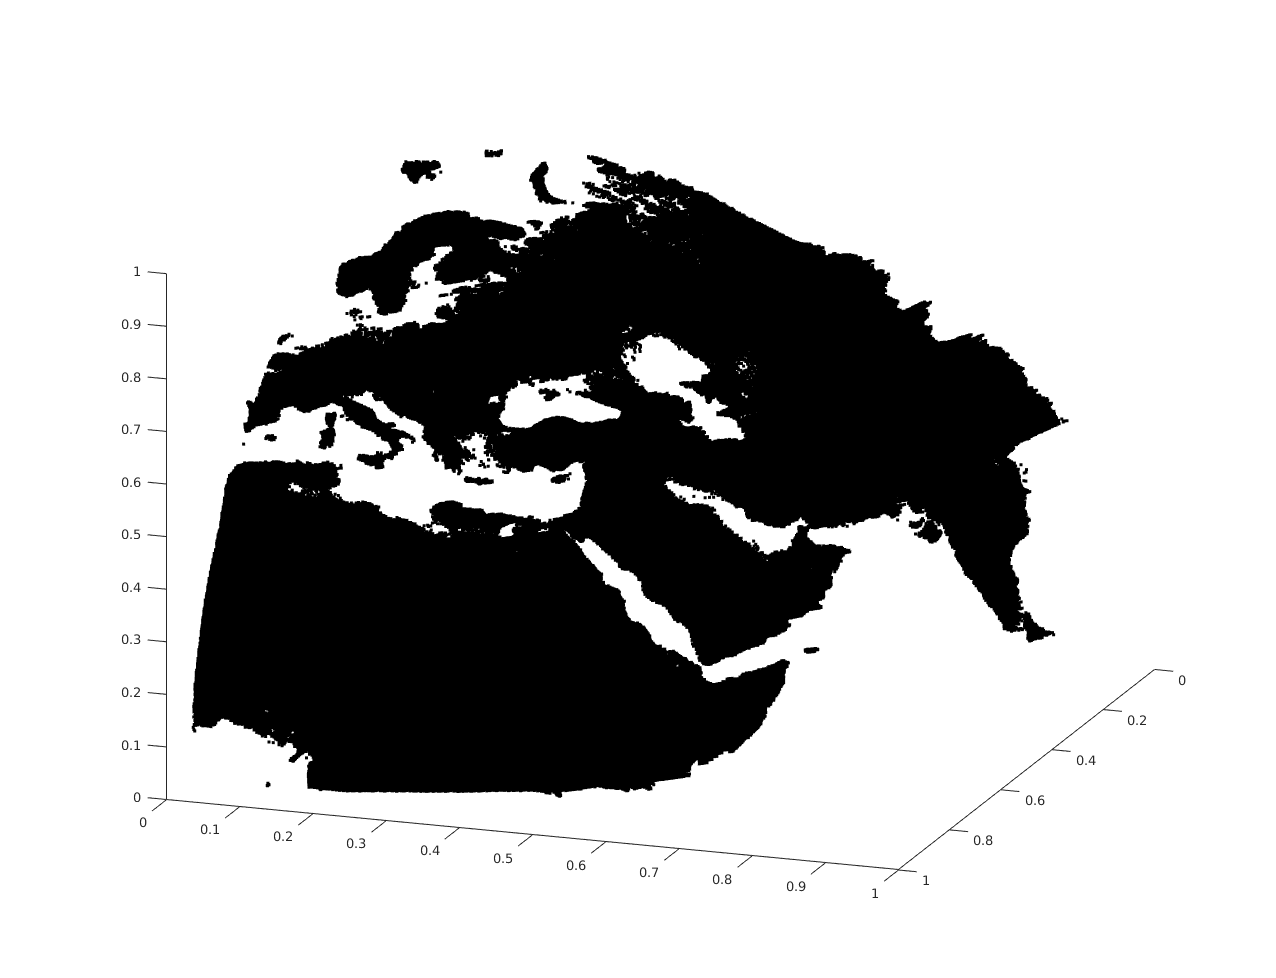
\includegraphics[width=\linewidth]{europe.png}
	\caption{Middle East and Europe, represented by 1 138 095 nodes after 20 repelling iterations; K=20. Altitudes are exaggerated by a factor of 100. The total running time was 238.292 seconds.}
	\label{europe}
\end{figure}



\begin{figure}[h!]
	\centering
	\begin{subfigure}{\linewidth}
	\includegraphics[width=\linewidth]{histogram_europe.png}
		%        \caption{cc}
	\end{subfigure}
%	\hskip2em
	\begin{subfigure}{\linewidth}
	\includegraphics[width=\linewidth]{greece.png}
		%        \caption{bb}
	\end{subfigure}
	\caption{Above, the histogram of the nearest neighbor distribution before(blue) and after (red) the repelling procedure. Below, a fragment of Greece.} 
	\label{fig:mult}
\end{figure}

\section{GPU implementation}



\section{Future work}

\begin{itemize}
\item The generation of the lattice on each box should be improved. We are working on transforming the lattice so that the density varies linearly within each box. This would make the density of the initial point generation more accurate and fewer repulsion steps would be needed.
\item Ideally the node distribution restricted to the boundary should be a reasonable 2D node distribution of variable density.
\item GPU-version of the ``main'' part \cite{Recipes1989}
\end{itemize}

\bibliography{nodes}
\bibliographystyle{plain}

\end{document}
